\documentclass[12pt, a4paper]{article}
\setlength{\parindent}{0pt}
\usepackage[utf8]{inputenc}
\usepackage[spanish]{babel}
\usepackage{hyperref}
\usepackage{graphicx}
\usepackage{wrapfig}
\usepackage{caption}
\usepackage{subcaption}
\usepackage{multirow} 
\usepackage{ amssymb }

\begin{document} 
\title{Trabajo Práctico 1\\ Machine Learning} 
\author{Bianchi, Gabina Luz} 
\maketitle
\section*{Ejercicio 4}

En este ejercicio se trabaja sobre el conjunto de datos de espirales anidadas. Se pide comparar las predicciones de los árboles generados con distinta cantidad de puntos de entrenamiento (150, 600 y 3000), sobre un conjunto de test de 10000 puntos. En la Figura 1 se grafican las tres predicciones.

\smallskip

En este caso es importante tener en cuenta que las variables X e Y del dataset son continuas. Por lo tanto, el algoritmo utilizado (c4.5), las discretiza para poder construir el árbol. Esto lo hace preguntándose en cada nodo, si alguna de las variables es mayor que cierto número elegido adecuadamente. De este modo, una variable X continua se discretiza en X \textgreater c o X $\geq$ c, evaluándose a dos posibles resultados: verdadero o falso. \\
Por ejemplo, el árbol construído con un conjunto de entrenamiento de 150 puntos, únicamente evalúa si Y $\leq$ 0.851042, siendo un árbol de solo 3 nodos. Naturalmente, esa no es una buena regla de clasificación para el data set utilizado, como se puede observar en la Figura 1 (a).

\smallskip

Las predicciones mejoran cuando se utilizan los conjuntos de entrenamientos más grandes, ya que se generan árboles de decisión más complejos en donde se tienen en cuenta ambas variables y para distintos valores. Sin embargo, en ambos casos se nota que las clases no están definidas por una curva si no que tienen terminaciones rectas, generadas justamente por la discretización de las variables.

\smallskip
Por otro lado, en el caso del árbol de decisión construído con un conjunto de entrenamiento de 3000 puntos, el error en el conjunto de test es mucho mayor al del conjunto de entrenamiento. Considerando esto y que el árbol construído es complejo, es posible que se esté produciendo sobreajuste. 



\begin{figure}
    \centering

    \begin{subfigure}[b]{0.45\textwidth}
        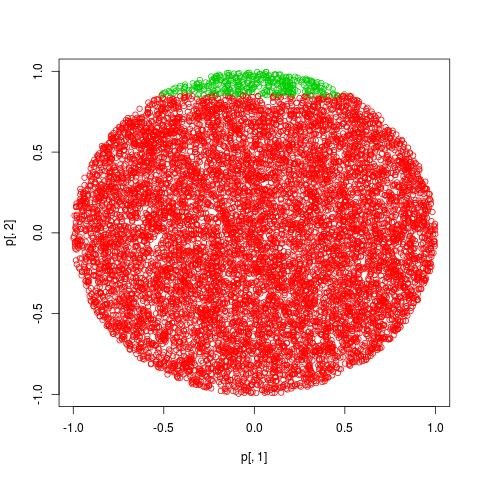
\includegraphics[width=\textwidth]{espirales150}
        \caption{150 puntos}
        %\label{fig:tiger}
    \end{subfigure}
      ~ %add desired spacing between images, e. g. ~, \quad, \qquad, \hfill etc. 
      %(or a blank line to force the subfigure onto a new line)
    \begin{subfigure}[b]{0.45\textwidth}
        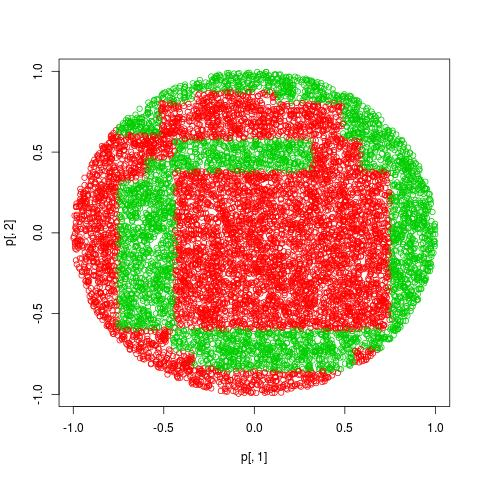
\includegraphics[width=\textwidth]{espirales600}
        \caption{600 puntos}
        %\label{fig:gull}
    \end{subfigure}
    ~ %add desired spacing between images, e. g. ~, \quad, \qquad, \hfill etc. 
      %(or a blank line to force the subfigure onto a new line)
    \begin{subfigure}[b]{0.45\textwidth}
        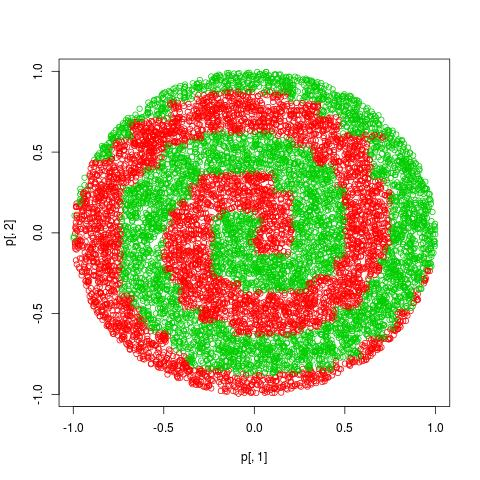
\includegraphics[width=\textwidth]{espirales3000}
        \caption{3000 puntos}
        %\label{fig:tiger}
    \end{subfigure}
    \caption{Gráficas de las predicciones para espirales anidadas según la cantidad de puntos de entrenamiento.}
\end{figure}


\section*{Ejercicio 5}
 En este ejercicio se trabaja sobre los conjuntos de datos gausianas diagonales y paralelas. Se pide comparar los errores porcentuales y los tamaños de los árboles generados a partir de conjuntos de entrenamiento de distinta longitud (100, 200, 300, 500, 1000 y 5000), considerando los datos antes y después de podar el árbol.

\bigskip

En este ejercicio se hace nuevamente una discretización de las variables, ya que todas las variables de las gausianas (en este caso X e Y), son continuas.

\medskip

Respecto a eso hay que tener en cuenta las diferencias que existen entre las dos bases de datos consideradas. En el caso de los datos diagonales la idea de partir las clases en función de si los valores de X e Y son mayores o menores a ciertos rangos, es aceptable. Las gausianas diagonales están justamente en cuadrantes opuestos. 
\\ Por el contrario, en los datos paralelos, el valor de Y no aporta ninguna información real para determinar a qué clase pertenece un punto. Si es tenida en cuenta, complejizará el árbol sin mejorar las predicciones. Esta idea se vuelve a analizar con más dimensiones en el ejercicio 7.\\
El razonamiento anterior se puede observar, por ejemplo en la Figura 2, en donde se graficaron las predicciones generadas al procesar el conjunto de test a partir de un conjunto de entrenamiento de longitud 100.
\\ Sin embargo, revisando los árboles generados, se puede notar que los casos en los que esto ocurre son lo menos.

\medskip

Otro aspecto a tener en cuenta es la tendencia que tienen los árboles de decisión en las distintas bases de datos. En la Figura 3 se graficaron las predicciones generadas al procesar el conjunto de test con el árbol de decisión construído a partir de un conjunto de entrenamiento de 5000 puntos para ambas gausianas. \\
Allí se puede observar que para la base de datos paralela la forma de clasificación es muy simple (y no solo eso, si no que es la correcta). Únicamente se evalúa si el punto está a la derecha o a la izquierda de la recta paralela al eje Y que pasa por el origen de coordenadas.\\
Esto explica por qué el árbol no tiende a crecer cuando el conjunto de entrenamiento es mayor, lo cual se puede observar en la Figura 6 (b).\\
Al observar la Figura 3 (a) se puede notar que el algoritmo no tiene la misma facilidad para resolver la clasificación en el caso de las gausianas diagonales. En lugar de hacer una división con una línea recta diagonal (que sería lo óptimo), lo hace escalonadamente. Debido a la forma en que analiza las variables cuando las discretiza, el algoritmo es incapaz de hacer cortes rectos y diagonales. Al aumentar la cantidad de puntos de entrenamiento con los cuales se genera el árbol, la cantidad de \textquotedblleft escalones \textquotedblright aumenta, intentando hacer el trazado diagonal. Esto explica la tendencia del árbol a crecer que se puede observar en la Figura 4 (b).\\
A su vez este razonamiento explica por qué la predicción es mejor para las gausianas paralelas que para las diagonales, lo cual se puede observar si se comparan la Figura 4 (a) y la Figura 6 (a).

\bigskip

El prunning es utilizado como un mecanismo para evitar el sobreajuste en las predicciones. Puede ocurrir que los datos del conjunto de entrenamiento tengan ruido, o aún sin tener ruido, muestren relaciones entre variables que no son generalizables al caso creal (sobre todo si el conjunto de entrenamiento es relativamente chico). La técnica de podar el árbol intenta eliminar aquellos errores.\\
Por lo tanto, lo esperable es que el error de entrenamiento aumente luego de podar el árbol, mientras que el error de test disminuya. De hecho, esto es lo que ocurre en ambos casos. Sin embargo, si se observan la Figura 5 (a) y la Figura 7 (a), comparadas con la Figura 4 (a) y la Figura 6 (a), respectivamente, las gráficas son muy similares.
\\ Para el caso de las gausianas paralelas, la similitud entre los errores porcentuales, antes y después de podar el árbol, se explica porque el algoritmo tiene una tendencia a resolver el problema correctamente. En general, se puede decir que no hace sobreajuste. Esto es analizado con mayor profundidad en el Ejercicio 6, a través del clasificador ideal. 
\\ Para el caso de las gausianas diagonales, si bien posiblemente se esté haciendo sobreajuste al momento de trazar dónde está cada "escalón" (ver Figura 3 (a)), el simplificar el árbol no mejora sustancialmente las predicciones, porque justamente el algoritmo es incapaz de resolver el problema correctamente.

\medskip

Respecto a la cantidad de nodos en el árbol, naturalmente, es esperable que en general disminuya luego de ser podado el árbol, como se observa si se comparan la Figura 4 (b) y la Figura 6 (b), con la Figura 5 (b) y la Figura 7 (b), respectivamente.\\
Se puede notar también, que para el caso de las gausianas paralelas con conjunto de entrenamiento de longitud 5000, la cantidad de nodos no disminye al podar el árbol. Esto sucede porque justamente, el tamaño es 3 nodos, habiéndo llegado a la clasificación ideal.

\begin{figure}
    \centering
	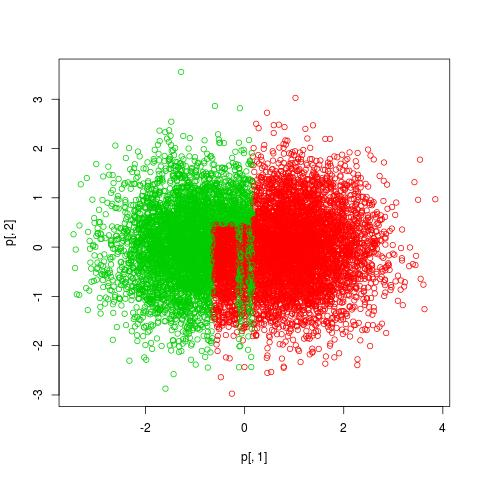
\includegraphics[scale=0.50]{gausianasB5}
	\caption{Gausianas paralelas utilizando un conjunto de entrenamiento de longitud 100.}


    \centering

    \begin{subfigure}[b]{0.45\textwidth}
        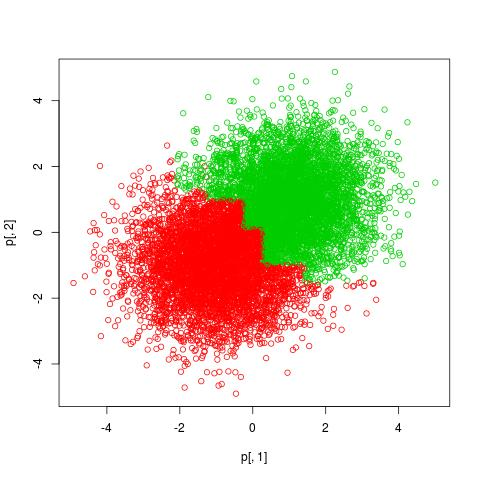
\includegraphics[width=\textwidth]{gausianasA}
        \caption{Gausianas diagonales.}
        %\label{fig:tiger}
    \end{subfigure}
      ~ %add desired spacing between images, e. g. ~, \quad, \qquad, \hfill etc. 
      %(or a blank line to force the subfigure onto a new line)
    \begin{subfigure}[b]{0.45\textwidth}
        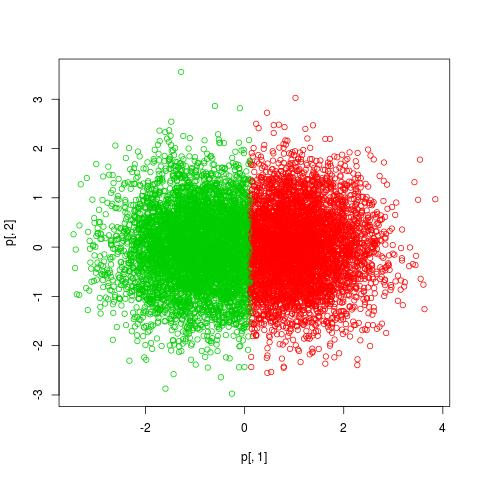
\includegraphics[width=\textwidth]{gausianasB}
        \caption{Gausianas paralelas.}
        %\label{fig:gull}
    \end{subfigure}
    \caption{Predicciones generadas al procesar el conjunto de test a partir de un conjunto de entrenamiento de longitud 5000 para ambas gausianas.}
\end{figure}


\begin{figure}
    \centering

    \begin{subfigure}[b]{0.65\textwidth}
        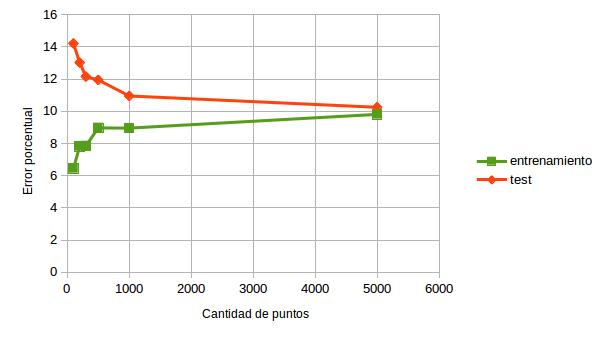
\includegraphics[width=\textwidth]{errorBA}
        \caption{Error porcentual en función de la cantidad de puntos de entrenamiento utilizados}
        %\label{fig:tiger}
    \end{subfigure}
      ~ %add desired spacing between images, e. g. ~, \quad, \qquad, \hfill etc. 
      %(or a blank line to force the subfigure onto a new line)
    \begin{subfigure}[b]{0.65\textwidth}
        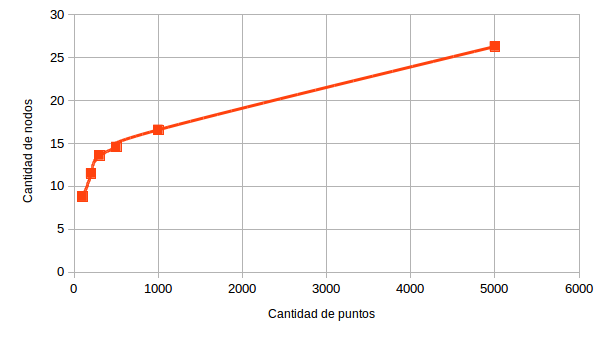
\includegraphics[width=\textwidth]{sizeBA}
        \caption{Tamaño del árbol en función de la cantidad de puntos de entrenamiento utilizados}
        %\label{fig:gull}
    \end{subfigure}
    \caption{Gráficas realizadas con los datos diagonales antes de podar el árbol}
\end{figure}


\begin{figure}
    \centering

    \begin{subfigure}[b]{0.65\textwidth}
        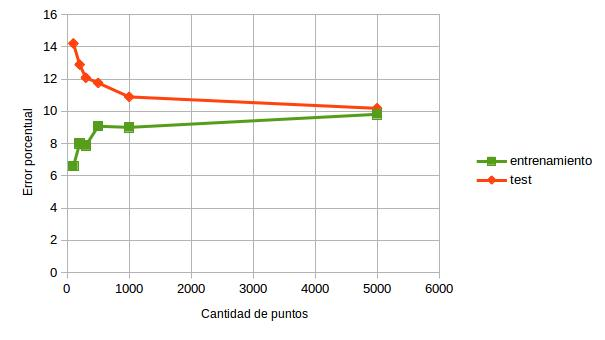
\includegraphics[width=\textwidth]{errorAA}
        \caption{Error porcentual en función de la cantidad de puntos de entrenamiento utilizados}
        %\label{fig:tiger}
    \end{subfigure}
      ~ %add desired spacing between images, e. g. ~, \quad, \qquad, \hfill etc. 
      %(or a blank line to force the subfigure onto a new line)
    \begin{subfigure}[b]{0.65\textwidth}
        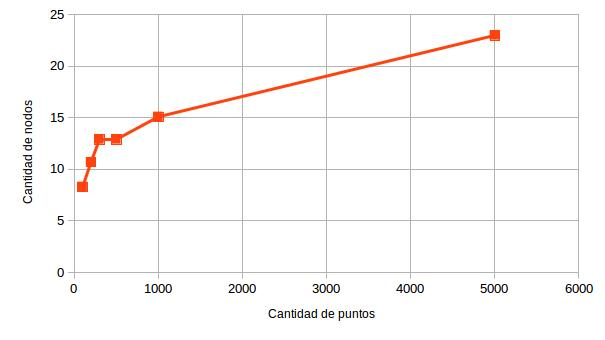
\includegraphics[width=\textwidth]{sizeAA}
        \caption{Tamaño del árbol en función de la cantidad de puntos de entrenamiento utilizados}
        %\label{fig:gull}
    \end{subfigure}
    \caption{Gráficas realizadas con los datos diagonales luego de podar el árbol}
\end{figure}


\begin{figure}
    \centering

    \begin{subfigure}[b]{0.65\textwidth}
        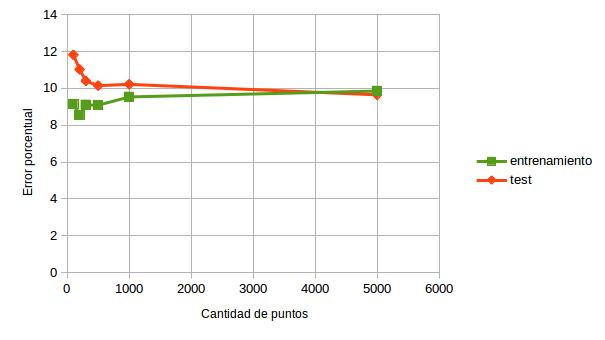
\includegraphics[width=\textwidth]{errorBB}
        \caption{Error porcentual en función de la cantidad de puntos de entrenamiento utilizados}
        %\label{fig:tiger}
    \end{subfigure}
      ~ %add desired spacing between images, e. g. ~, \quad, \qquad, \hfill etc. 
      %(or a blank line to force the subfigure onto a new line)
    \begin{subfigure}[b]{0.65\textwidth}
        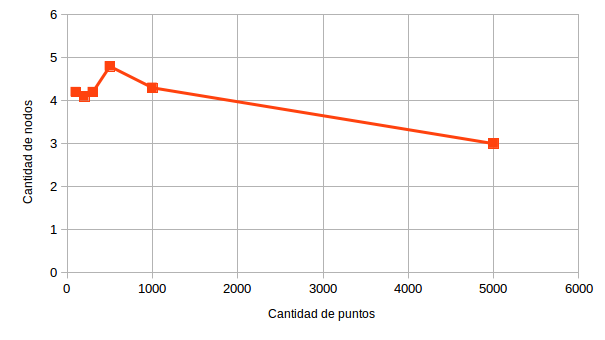
\includegraphics[width=\textwidth]{sizeBB}
        \caption{Tamaño del árbol en función de la cantidad de puntos de entrenamiento utilizados}
        %\label{fig:gull}
    \end{subfigure}
    \caption{Gráficas realizadas con los datos paralelos antes de podar el árbol}
\end{figure}


\begin{figure}
    \centering

    \begin{subfigure}[b]{0.65\textwidth}
        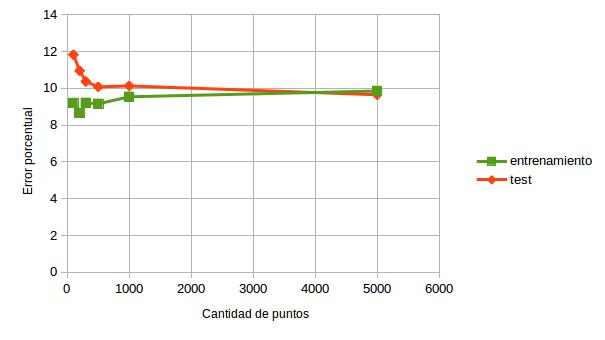
\includegraphics[width=\textwidth]{errorAB}
        \caption{Error porcentual en función de la cantidad de puntos de entrenamiento utilizados}
        %\label{fig:tiger}
    \end{subfigure}
      ~ %add desired spacing between images, e. g. ~, \quad, \qquad, \hfill etc. 
      %(or a blank line to force the subfigure onto a new line)
    \begin{subfigure}[b]{0.65\textwidth}
        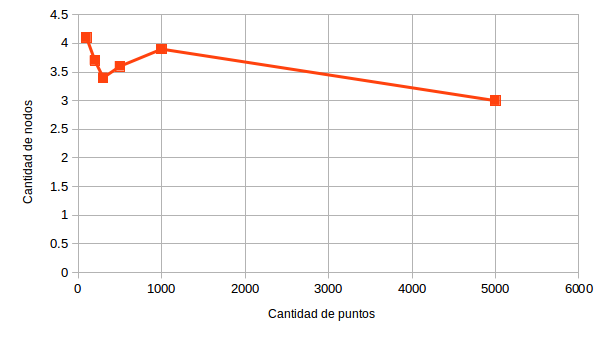
\includegraphics[width=\textwidth]{sizeAB}
        \caption{Tamaño del árbol en función de la cantidad de puntos de entrenamiento utilizados}
        %\label{fig:gull}
    \end{subfigure}
    \caption{Gráficas realizadas con los datos paralelos luego de podar el árbol}
\end{figure}

\section*{Ejercicio 6}
En el ejercicio 6 se pide comparar los errores de test porcentuales de ambas gausianas cuando se varía el C. 

\bigskip

Considerando que el C está relacionado directamente con cuánto se solapan las clases, es esperable que, a medida que aumente el C (si todas las otras variables quedan fijas), aumente el error porcentual.

\bigskip

A su vez, es posible determinar cuál es el error mínimo de clasificación para cada valor de C. Esto lo podemos lograr sencillamente si utilizamos el clasificador ideal para este tipo de problema. \\
La idea del clasificador ideal es simple: primero es necesario determinar los centros de las gausianas, después para cada punto a clasificar se calcula la distancia euclidiana a los dos centros, finalmente se elige la clase cuyo centro sea el más cercano a dicho punto. En caso de que el punto sea equidistante a ambos centros, se elige una clase de manera aleatoria.

\bigskip

Para el caso de las gausianas paralelas, al comparar los errores porcentuales generados con las predicciones del algoritmo c4.5 con los errores generados con el clasificador ideal, es esperable que dichas curvas sean parecidas. Justamente, como se observó en el ejercicio 5, el algoritmo tiende a clasificar correctamente el problema de las gausianas paralelas (para 2 dimensiones, y con un conjunto de entrenamiento de 5000 puntos). Sin embargo, es esperable que el error producido por el c4.5 sea mayor que el ideal, ya que el conjunto de entrenamiento utilizado es relativamente chico comparado con la cantidad de dimensiones (250 y 5, respectivamente).

\bigskip

En el caso de las gausianas diagonales, considerando que el algoritmo es incapaz de resolver el problema de forma óptima (como se vio en el ejercicio 5), es esperable que la curva de error producida por c4.5 esté por encima que la producida por el clasificador ideal.

\smallskip

Todo lo analizado anteriormente se puede observar en la Figura 8.


\begin{figure}
    \centering
	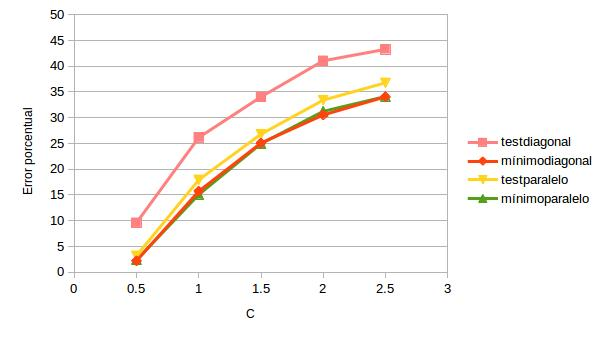
\includegraphics[scale=0.70]{ejercicio6}
	\caption{Errores porcentuales de test y mínimos para ambas gausianas en función de C.}
\end{figure}

\section*{Ejercicio 7}
En el ejercicio 7 se pide comparar los errores de entrenamiento y test porcentuales de ambas gausianas cuando se varía la cantidad de dimensiones. 


\bigskip

Una cuestión a analizar es cuáles variables aportan información útil en cada caso. Independientemente de la cantidad de dimensiones que haya, en el caso de las gausianas paralelas, se deberá tener en cuenta únicamente la primera variable. Las otras variables pordrían ser consideradas ruido. Por el contrario, en el caso de las gausianas diagonales, todas las variables aportan información útil.  

\bigskip

Si se observan los árboles de decisión generados para las gausianas paralelas, se puede notar que en muchos de ellos se considera a más de una variable. Es decir, las dimensiones tienden a confundir al algoritmo y agrandar los árboles con ruido. Debido a esto es que a medida que aumenta la cantidad de dimensiones, el sobreajuste es mayor: el error de entrenamiento disminuye mientras que el de test aumenta y, por lo tanto, la diferencia entre éstos se agranda.

\bigskip

El caso de las gausianas diagonales no es fácil de resolver para este algoritmo. El conjunto de datos particular con dos dimensiones fue analizado en el ejercicio 5. Al aumentar las dimensiones, aumenta la complejidad ya que más variables deben ser tenidas en cuenta. A su vez, la cantidad de puntos utilizados para generar los árboles de decisión es constante y relativamente pequeña en comparación con la cantidad de dimensiones. Debido a esto es esperable que se produzca cada vez más sobreajuste: se encuentran relaciones entre las variables que no son reales, y por lo tanto, el error de entrenamiento es muy bajo y el de test, muy alto.

\bigskip

Todo lo analizado anteriormente se puede observar en la Figura 9.

\begin{figure}
    \centering
	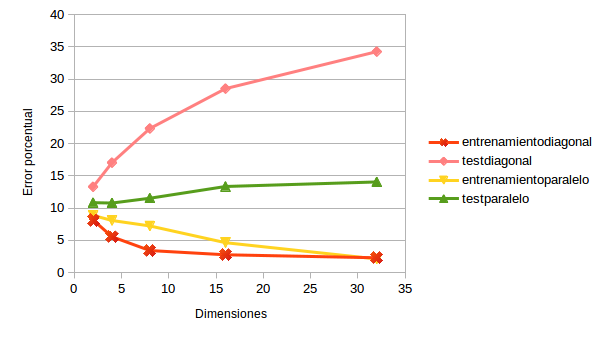
\includegraphics[scale=0.70]{ejercicio7}
	\caption{Errores porcentuales de entrenamiento y test para ambas gausianas en función de la cantidad de dimensiones.}
\end{figure}

\subsection*{Ejercicio 8}
En este ejercicio se pide hacer un análisis sobre el problema XOR. En la Figura 10 se grafican las clases.

\bigskip

Observando el problema, la clasificación más sencilla para resolverlo es la siguiente. 
\begin{verbatim}
- X < 0
    - Y < 0 : 1
    - Y >= 0 : 0
- X >= 0
    - Y < 0 : 0
    - Y >= 0 : 1
\end{verbatim}

Sin embargo, al procesar los datos con el algoritmo c4.5, éste nos devuelve un árbol de un único nodo. Es decir, clasifica todos los puntos como una única clase. \\
Esto ocurre por la forma en que el algoritmo analiza las variables. Utiliza un algoritmo greedy en el cual en cada caso se queda con la variable que separa mejor las clases. El problema es que en la base de datos XOR ninguna de las variables da alguna información por sí sola, es necesario considerarlas a las dos juntas. Por lo tanto, al intentar elegir cuál variable será la raíz del árbol de decisión, analiza cada variable por separado y ninguna le aporta información. De ese modo, devuelve un árbol de un único nodo, en donde todos los puntos pertenecen a la misma clase. 

\begin{figure}
    \centering
	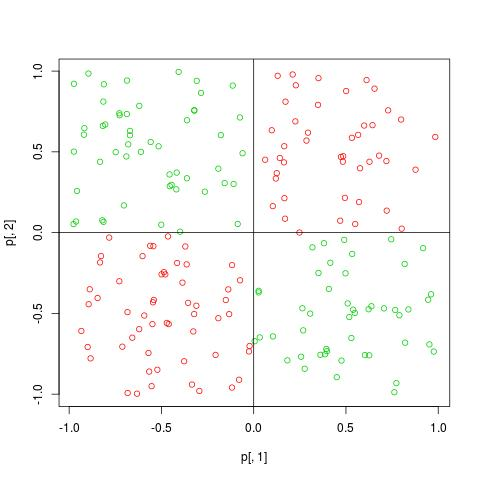
\includegraphics[scale=0.50]{ejercicio8}
	\caption{Clases de XOR}
\end{figure}


\end{document}


